\apendice{Documentación técnica de programación}

\section{Introducción}
En este apartado se detallará cómo entrenar nuestros agentes inteligentes y como hacerlos funcionar en el entorno del videojuego. Hay que recalca que ha sido necesario crear dos implementaciones muy similares pero diferentes, ya que uno de los problemas era de tipo \emph{multilabel} y el otro era de tipo \emph{multiclase}.

\section{Estructura de directorios}
A continuación se va a explicar la estructura de directorios para no perder el tiempo buscándolo todo.

Los principales directorios del proyecto son:
\begin{itemize}
    \item Proyectos Unity
    \item Redes Neuronales
    \item DecicionTreeClasiffiers
    \item Ejemplos y pruebas
\end{itemize}

En el directorio de «proyectos Unity»  encontraremos los dos principales proyectos de videojuego con los que se ha trabajado. En primer lugar podemos encontrar el proyecto «Juego». Este proyecto contiene el juego principal, el que van a utilizar los usuarios para obtener los datos de las partidas. Por otro lado tenemos el proyecto «Juego\_lite». Esta segunda versión de la implementación es una versión reducida del primero, carece de menús y sonido, ya que únicamente está destinado a ser jugado por la máquina. Finalmente tenemos un último directorio en el que encontramos los proyectos de que probaban funcionalidades muy concretas, como las pruebas de conexión de sockets y el lanzamiento del juego con parámetros desde terminal.

En los directorio «DecsionTreeClasiffiers» y «RedesNeuronales», encontramos una \empg{build} del juego lista para funcionar, cada una referente a su tipo de algorimo. Los scripts de Python deben ir dentro del directorio AI\_Data y los modelos entrenados los he colocado junto al ejecutable pero, como se va a referenciar con una ruta relativa, se pueden colocar donde más nos guste. Junto al ejecutable he creado un acceso directo al mismo, esto es porque el juego ha de lanzarse con parámetros y esto nos facilita la tarea.

Como es de esperar, la realización de este proyecto ha requerido de una gran labor de investigación, síntesis y pruebas. En el directorio pruebas y ejemplos podemos encontrar un «batiburrillo» de ejemplos realizados con ayuda del tutor y apuntes de la asignatura de «Minería de datos». Además, se han guardado en ésta carpeta varios sets de datos antiguos que fueron utilizados en las primeras pruebas.


\section{Manual del programador}
Voy a proceder a explicar cómo se debería proceder para la compilación del juego, entrenamiento de los agentes inteligentes y su posterior uso.


\section{Compilación, instalación y ejecución del proyecto}
Como que este proyecto esta dividido en tantas partes empezaré explicando cómo instalar python, qué bibliotecas necesitamos y cómo se instalan.

\subsection{Instalando Python}

Este royecto ha sido realizado utilizando \emph{Anaconda}\footnote{\url{https://www.continuum.io/downloads}}, una distribución de \emph{Python}. Para obtener \emph{Anaconda} vamos a su página web y descargamos la versión correspondiente a nuestro sistema operativo(32/64 bits). 

\begin{figure}[h!]
    \centering
    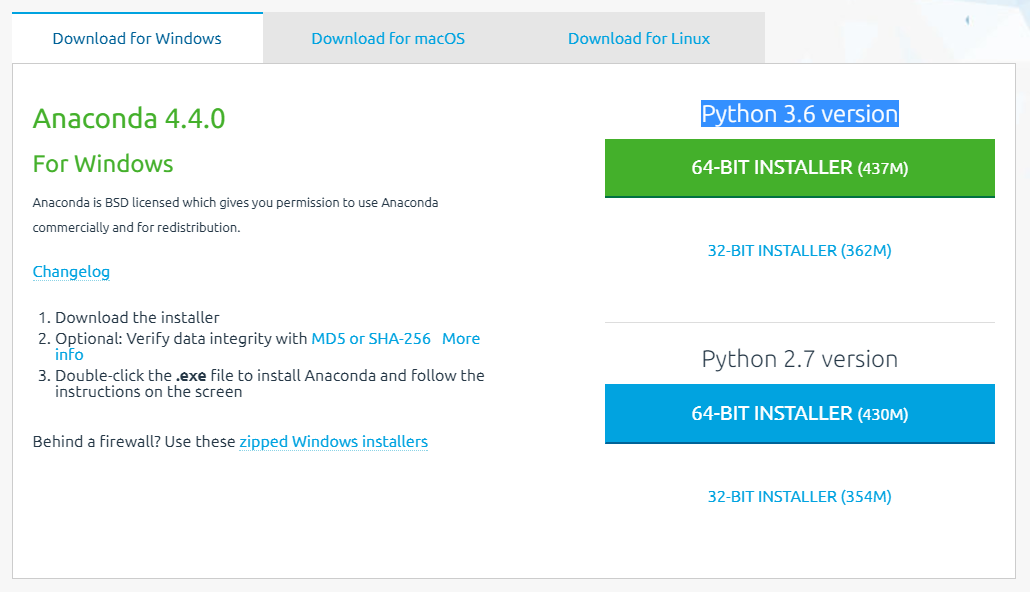
\includegraphics[width=\textwidth]{descargaPython}
    \caption{Descarga Anaconda}
    \label{fig:anaconda}
\end{figure}


IMPORTANTE: Actualmente hay varias versiones disponibles de Python. A lo largo de este proyecto se ha utilizado la 3.5.2, que sería compatible con cualquier versión a partir de la 3.0, pero incompatible con cualquier versión inferior \ref{fig:anaconda}.

Una vez instalado anaconda procedemos a instalar los paquetes necesarios para los scripts. \emph{Anaconda} trae por defecto muchos paquetes de los que necesitamos, ente los que están: 
\begin{itemize}
    \item NumPy.
    \item pandas.
    \item SciPy.
    \item Matplotlib.
    \item Jupyter.
\end{itemize}

Además de estos paquetes, necesitaremos \emph{Pickle} y \emph{Deap}. La instalación de paquetes en \emph{Anaconda} es sumamente sencilla. Abrimos el terminal de windows y escribimos:

\colorbox{black}{\textcolor{white}{conda install package-name}}


Cuando termine de instalar deberíamos tener el entorno de  listo para trabajar en él.

\subsection{Instalando Unity3D}

Para cargar y compilar el juego necesitaremos Unity3D. Es software de desarrollo de videojuegos se puede descargar gratuitamente desde su página web. \url{https://unity3d.com/es/get-unity/download}

\begin{figure}[h!]
    \centering
    
\includegraphics[width=\textwidth]{UnityInstall}
    \caption{Descarga Unity3D}
    \label{fig:Unity}
\end{figure}

Para este proyecto es suficiente con descargar la versión gratuita. Ejecutamos el instalador y elegimos la opción por defecto. En una de las pantallas nos permite seleccionar qué componentes se quiere instalar, con seleccionar los que se ven en \ref{fig:Unity2} es suficiente.

\begin{figure}[h!]
    \centering
    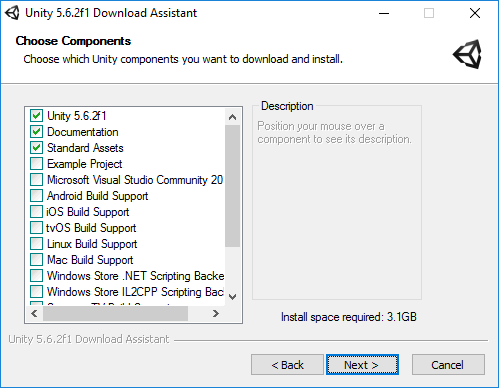
\includegraphics[width=0.5\textwidth]{UnityInstall2}
    \caption{Descarga Unity3D}
    \label{fig:Unity2}
\end{figure}


\subsection{Compilación}
Para la compilación del juego hay que ejecutar Unity3D y cargar el proyecto que se va a compilar. Para ello se han de seguir los siguientes pasos:
\begin{itemize}
    \item 1 - Lanzar Unity3D y cargar el proyecto. Al lanzar Unity3D, si no hemos modificado ninguna configuración, nos debe mostrar una ventana como \ref{fig:compile1}. En esta ventana nos muestra los proyectos recientes que, si es la primera vez que lo lanzamos, estará vacía. Para cargar un proyecto no listado pulsamos el botón «Open» y buscamos el proyecto en nuestro disco. En este caso hay que cargar el que he denominado «Juego».
        \begin{figure}[h!]
        \centering
        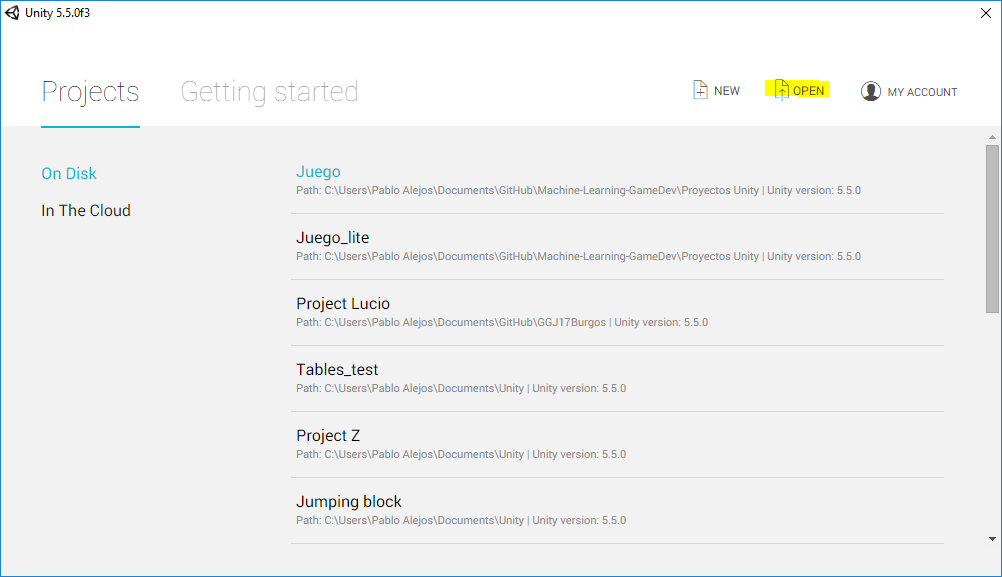
\includegraphics[width=\textwidth]{Compile1}
        \caption{Carga proyecto Unity3D}
        \label{fig:compile1}
        \end{figure}
\item 2- Compilación del juego. Para compilar el juego vamos a «File» > «Build settings» y se nos abre la ventana de compilación \ref{fig:compile3}.
        \begin{figure}[h!]
        \centering
        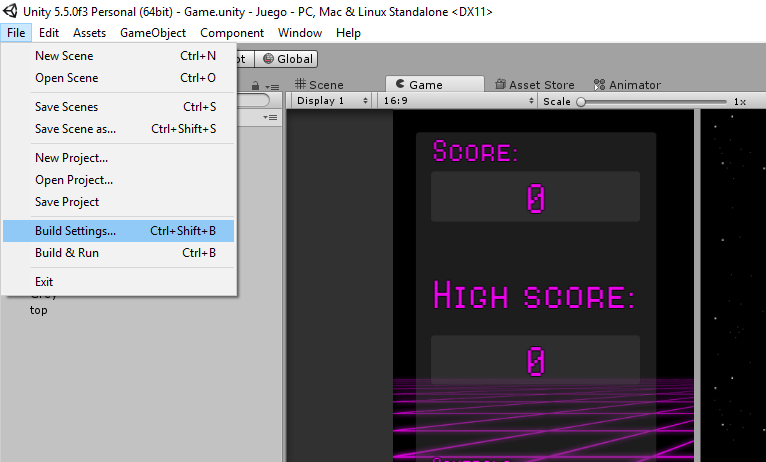
\includegraphics[width=\textwidth]{Compile2}
        \caption{Compilar proyecto}
        \label{fig:compile2}
        \end{figure}
En la ventana de compilación deberían aparecer cargadas dos escenas, identificadas con el id 0 y 1 respectivamente. Hecha esta comprobación procedemos con la \emph{build}. Para compilar el juego pulsamos sobre build y seleccionamos la carpeta donde lo queremos guardar.
        \begin{figure}[h!]
        \centering
        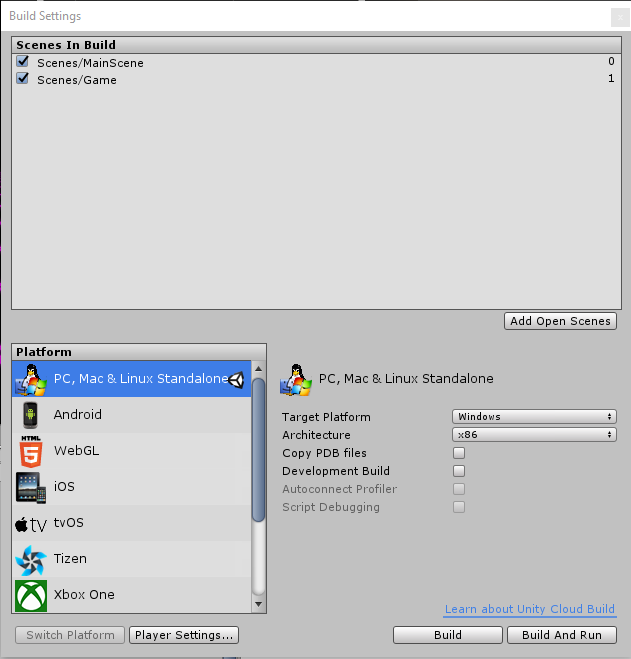
\includegraphics[width=\textwidth]{Compile3}
        \caption{Ventana de compilación}
        \label{fig:compile3}
        \end{figure}
\end{itemize}

Con el juego ya compilado no tendríamos mas que entregar al jugador el ejecutable con las carpeta de binarios generada y este podría empezar a jugar y a generar datos. Mientras nuestro «sujeto de prueba» está entretenido jugando, vamos a continuar haciendo la build del juego que utilizará nuestro agente inteligente.



\subsection{Incorporación de los scripts}
En este punto ya tenemos \emph{Python} instalado, Unity3D instalado y hemos creado una build del juego.

Para la compilación del juego reducido, el juego que utilizarán los agentes inteligentes se siguen los mismos pasos mencionados anteriormente, pero esta vez cargaremos el proyecto denominado «Juego\_lite». Esta es una versión reducida del juego, no dispone de menú principal y de ha eliminado la banda sonora.

Una vez compilado debemos añadir a la build los scripts de python. Los scripts de python se encuentran el la carpeta «Scripts\_python» que cuelga de la raíz principal y elegimos los correspondientes al tipo de agente inteligente que queremos utilizar. Disponemos de los scripts relativos a los arboles de decisión, o bien, de los relativos a las redes neuronales. Una vez seleccionados los scripts de Python que necesitamos, se copian en la carpeta «AI\_Data» que acompaña al ejecutable.

Ya tenemos listo el entorno en el que vamos a probar los modelos entrenados.



\subsection{Guía de uso para árboles de decisión}


\textbf{Entrenamiento}

Para entrenar un modelo necesitamos dos cosas, el script llamado «trainer.py» y el dataset en formato $csv$, ambos han de estar en la misma carpeta. El entrenamiento es tan sencillo como abrir la linea de comandos de \emph{windows}, ir a la carpeta en la que tengamos el script y el dataset y escribir:

\colorbox{black}{\textcolor{white}{python trainer.py}}

Este comando ejecutará automáticamente un entrenamiento con el modelos por defecto (Decision tree).

Este script nos permite seleccionar el tipo de clasificador que queremos utilizar y con qué nombre lo vamos a guardar. en primer lugar se debe especificar el nombre del clasificador \emph{RandomForestClassifier} o bien, \emph{DecisionTreeClassifier}. En segundo lugar podemos especificar el nombre del fichero en el que lo vamos a guardar. Un ejemplo de ejecución sería:


\colorbox{black}{\textcolor{white}{python trainer.py RandomForestClassifier rfc.sav}}

Este comando nos entrenaría un modelo empleando un random forest classifier y lo salvaría en el fichero rfc.sav.

\textbf{Ejecución}

Para lanzar el ejecutable haciendo uso un modelo entrenado tenemos varias opciones:

Una opción es abrir la consola de windows, ir hasta la carpeta que contiene el ejecutable y escribir:

\colorbox{black}{\textcolor{white}{AI.exe nro\_de\_rondas tiempo\_de\_ronda ruta\_relativa\_del\_modelo}}

\textbf{Todos los parámetros son obligatorios}.

Otra forma de ejecutar el juego utilizando parámetros es crear un acceso:

\begin{figure}[h!]
    \centering
    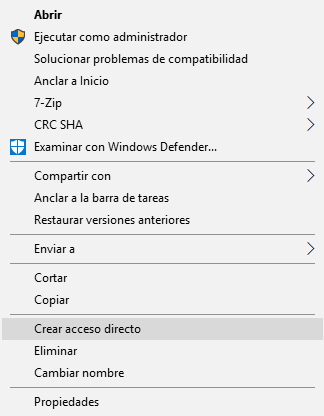
\includegraphics[width=0.5\textwidth]{accesoDirecto1}
    \caption{Creación de un acceso directo}
    \label{fig:accesoDirecto1}
\end{figure}


Una vez creado el acceso directo le hacemos clic derecho, propiedades y al final de la ruta escribimos los parámetros que le queremos aplicar como se puede ver en la figura \ref{fig:accesoDirecto2}. Una vez hecho esto, siempre que hagamos doble clic en el acceso directo se ejecutará con esos parámetros.


\begin{figure}[h!]
    \centering
    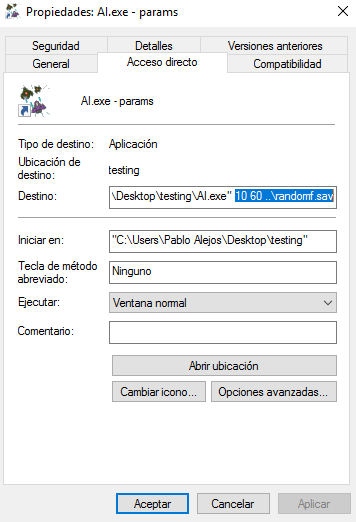
\includegraphics[width=0.5\textwidth]{accesoDirecto2}
    \caption{Parámetros de un acceso directo}
    \label{fig:accesoDirecto2}
\end{figure}

Si todo está correctamente configurado, al hacer doble clic en el acceso directo comenzará una partida y el modelo especificado comenzará a jugar.


\subsection{Guía de uso de redes neuronales}

En el caso de las redes neuronales, el entrenamiento y explotación tiene algo más de trabajo. Por este motivo, he decidido hacerlo en un libro de \emph{jupyter}.

En primer lugar hay que hacer una comprobación importante. \emph{Jupyter} utiliza también un tipo de socket para ejecutar sus servicios, y el puerto que utiliza es el 8888, el mismo que he estado yo utilizando para mis scripts. Este conflicto hace que tengamos que cambiar el puerto por defecto de \emph{Jupyter}, ya que cambiar el del juego es algo mas engorroso. Para cambiar el puerto de \emph{Jupyter} hay que seguir los siguientes pasos:
\begin{itemize}
    \item 1. Abrir una consola de Windows y escribir:
    
    \colorbox{black}{\textcolor{white}{jupyter notebook --generate-config}}
    
    Esto genera un fichero de configuración en la ruta por defecto de \emph{Jupyter} llamado jupyter\_notebook\_config.py.
    \item 2.Abrir el fichero que nos ha creado e ir a la línea que pone: 
    
    c.NotebookApp.port = 8888
    
    y cambiar el 8888 por 7777.
    \item Guardamos el fichero de configuración y lanzamos \emph{Jupyter}.
\end{itemize}

\textbf{Entrenamiento y explotación}
Abrimos el libro \emph{Jupyter} llamado «NeuralNetwork». Este notebook de \emph{Jupyter} se divide en varias secciones:
\begin{itemize}
    \item Carga de datos.
    \item Creación del \emph{pipeline} inicial.
    \item Neuroevolición
    \item Calibrado de parámetros
    \item Bot de Telegram
\end{itemize}

\textbf{Carga de datos}

Este tipo de entrenamiento podría empezar sin cargar datos pero, dado que ya disponemos de un gran conjunto de datos, vamos a aprovechar los datos de los que disponemos para preentrenar un perceptrón multicapa (MLP), de esta forma se pretende reducir el tiempo de entrenamiento. 

La carga de datos es sencilla. simplemente hay que ir ejecutando una a una las celdas hasta el pipeline.

En este punto tenemos dos opciones, generar un MLP con los parámetros por defecto o saltar momentáneamente al calibrado de parámetros.

\textbf{Calibrado de parámetros}
En este proyecto se ha implementado el método de calibrado mediante random\_search. Este método lo que hace es seleccionar una combinación aleatoria de entre las opciones que le da el programado y lo evalúa, al final, te dice cuál cree él que es la mejor combinación. Si se ponen demasiadas iteraciones puede tardar un buen rato, pero sabes que va a valorar más posibilidades y, por lo tanto, es más probable que de con un buen resultado.

\textbf{Creación del pipeline}
Con el calibrado hecho, establecemos los parámetros que el calibrado nos ha proporcionado y creamos el pipeline. Un pipeline es una sucesión de operaciones que se hacen a la hora de entrenar un modelos. Este pipeline se divide en etapas, en mi caso, solo tiene dos. La primera etapa es un Standard scaler, que me ajusta los datos a una escala de forma que los datos dispersos influyan un poco menos en el conjunto. La segunda etapa es el propio MLP. Ejecutamos la celda que contiene el pipeline y tendremos un fichero nuevo llamado «pipe.sav».


\textbf{Computación neuronal}
Para evolucionar el clasificador basta con ejecutal la celda que contiene el algoritmo evoulivo, aún así, explicaré brevemente qué es lo que hace:

Como ya se indicaba en la memoria, hay que definir la función de \emph{fitness}, el método que nos pasa de gen a coeficientes y viceversa y la población inicial. En la sección «neuroevolución» del notebook tenemos estos tres métodos que se llaman: \textbf{gen2Coefs} y \textbf{coefs2gen} para transformar el genoma, \textbf{MLPFitness} para el cálculo de valor de  \emph{fitness} e \textbf{initPopulation} para decir cómo ha de ser iniciarse la población inicial.

una vez definidos estos métodos hay que definir el algoritmo evolutivo. Para los algoritmos evolutivos se ha empleado la biblioteca \emph{Deap}. Para crear nuestro modelo de algoritmo evolutivo, Deap utiliza lo que denomina \emph{Toolbox}. Las \emph{Toolbox} de Deap contienen la información del evolutivo como, por ejemplo, tipo de individuos, codificación del individuo, forma de mutar, tipo de cruce, etc.

Con todos los parámetros definidos ya podemos empezar a evolucionar el clasificador. Para evolucionar el clasificador, Deap nos facilita varios modelos de algoritmos evolutivos, en este caso yo utilice \emph{eaSimple}, que es el que mas a aproxima al modelo explicado en Conceptos teóricos.


\section{Pruebas del sistema}
En el desarrollo de este proyecto, por desconocimiento del entorno de desarrollo no me sido posible realizar las pruebas automatizadas que me hubiera gustado. Por otro lado, se han realizados numerosas pruebas manuales en forma de pequeños test unitarios, con el fin de que me diesen una noción de que el funcionamiento era el esperado.



